\documentclass[11pt]{book}
\usepackage{gvv-book}
\usepackage{gvv}
\usepackage[sectionbib,authoryear]{natbib}
\setcounter{secnumdepth}{3}
\setcounter{tocdepth}{2}
\makeindex
\begin{document}
\frontmatter
\tableofcontents
\setcounter{page}{1}
\mainmatter
\chapter{Triangle}
Consider a triangle with vertices
\begin{align}
\label{eq:tri-pts}
\vec{A}=\myvec{-3 \\ 0},\,
\vec{B}=\myvec{4\\2},\,
	\vec{c}=\myvec{1\\4},\,
\end{align}
\section{Vectors}
\begin{enumerate}[label=\thesection.\arabic*.,ref=\thesection.\theenumi]
\numberwithin{equation}{enumi}

\item The direction vector of $AB$ is defined as
		\begin{align}
			\vec{B}-
			\vec{A}
		\end{align}
Consider a triangle with vertices
\begin{align} 
 \vec{A} &= \myvec{ -3\\ 0 } \\ \vec{B} &= \myvec{ 4\\ 2 }
  \\\vec{C} &= \myvec{ 1\\ 4}
 \end{align}
The Direction Vector of $AB$ is defined as 
\begin{align} 
\vec{B} - \vec{A}
\end{align}
Question1.1.1 :Find the Direction Vectors of $AB$,$BC$,$CA$.\\
\solution

\begin{enumerate} 
\item  The Direction vector of $AB$ is \begin{align} &= \vec{B} - \vec{A} \\
 &= \myvec{4 - (-3)\\ 2 - (0) } \\&= \myvec{ 7\\ 2 }
 \end{align}
 
\item The Direction vector of $BC$ \begin{align}&= \vec{C} - \vec{B}\\
 &= \myvec{ 1 - 4\\ 4 - 2 } \\&= \myvec{-3\\ 2 }
  \end{align}
  
  \item  The Direction vector of $CA$  \begin{align} &= \vec{A} - \vec{C} \\ 
 &= \myvec{ -3 - 1\\ 0 - (4) } \\&= \myvec{ -4\\ -4 }
  \end{align}
 \end{enumerate}

\item The length of side $BC$ is 
		\begin{align}
			\norm{\vec{B}-\vec{A}} \triangleq \sqrt{\brak{\vec{B}-\vec{A}}^{\top}{\vec{B}-\vec{A}}}
		\end{align}
		where
		\begin{align}
			\vec{A}^{\top}\triangleq\myvec{1 & 0}
		\end{align}
Question 1.1.2 : Find the length of side AB, BC, CA.\\
\solution
Solving for BC
Given, 
\begin{align}
\vec{A} = \myvec{-3\\0},
\vec{B} = \myvec{4\\2},
\vec{C} = \myvec{1\\4} \\  
 \norm{\vec{B}-\vec{C}}\ &=  \sqrt{\brak{\vec{B}-\vec{C}}^{\top}\brak{\vec{B}-\vec{C}}} \\
 \vec{B}-\vec{C} &= \myvec{4\\ 2} - \myvec{1 \\ 4} \\
 \vec{B}-\vec{C} &= \myvec{3\\ -2} \\
 \brak{\vec{B}-\vec{C}}^{\top} &= {\myvec{3\\ -2}}^{\top} = \myvec{3 \ -2} \\
\brak{\vec{B}-\vec{C}}^{\top}\brak{\vec{B}-\vec{C}} &= \myvec{3\ -2} \myvec{3 \\ -2}\\
             &= 9+4 \\
             &= 13 \\  
 \sqrt{\brak{\vec{B}-\vec{C}}^{\top}\brak{\vec{B}-\vec{C}}} &= \sqrt{13}	\\
	\implies \norm{\vec{B}-\vec{C}}\ &= \sqrt{13}
\end{align}

Solving for AB 
Given, 
\begin{align}  
 \norm{\vec{A}-\vec{B}}\ &=  \sqrt{\brak{\vec{A}-\vec{B}}^{\top}\brak{\vec{A}-\vec{B}}} \\
 \vec{A}-\vec{B} &= \myvec{-3\\ 0} - \myvec{4 \\ 2} \\
 \vec{A}-\vec{B} &= \myvec{-7 \\ -2} \\
 \brak{\vec{A}-\vec{B}}^{\top} &= {\myvec{-7 \\ -2}}^{\top} = \myvec{-7 \ -2} \\
\brak{\vec{A}-\vec{B}}^{\top}\brak{\vec{A}-\vec{B}} &= \myvec{-7 \ -2} \myvec{-7 \\ -2}\\
             &= 49 + 4 \\
             &= 53 \\  
	\sqrt{\brak{\vec{A}-\vec{B}}^{\top}\brak{\vec{A}-\vec{B}}} &= \sqrt{53}	\\
	\implies \norm{\vec{A}-\vec{B}}\ &= \sqrt{53} 
\end{align}

Solving for CA
Given, 
\begin{align}  
	\norm{\vec{C}-\vec{A}}\ &=  \sqrt{\brak{\vec{C}-\vec{A}}^{\top}\brak{\vec{C}-\vec{A}}} \\
 \vec{C}-\vec{A} &= \myvec{1 \\ 4} - \myvec{-3 \\ 0} \\
 \vec{C}-\vec{A} &= \myvec{4 \\ 4} \\
 \brak{\vec{C}-\vec{A}}^{\top} &= {\myvec{4 \\ 4}}^{\top} = \myvec{4 \ 4} \\
	\brak{\vec{C}-\vec{A}}^{\top}\brak{\vec{C}-\vec{A}} &= \myvec{4\ 4} \myvec{-4 \\ 4}\\
             &= 16 + 16 \\
             &= 32 \\  
	\sqrt{\brak{\vec{C}-\vec{A}}^{\top}\brak{\vec{C}-\vec{A}}} &= \sqrt{32}	\\
	\implies \norm{\vec{C}-\vec{A}}\ &= \sqrt{32} 
\end{align}



\item   Points $\vec{A}, \vec{B}, \vec{C}$ are defined to be collinear if 
		\begin{align}
			\rank{\myvec{1 & 1 & 1 \\ \vec{A}& \vec{B}&\vec{C}}} = 2
		\end{align}
Are the given points in
			\eqref{eq:tri-pts}
collinear?\\
Question 1.1.3 : Check the collinearity of $\vec{A},\vec{B},\vec{C}$ \\ 
\solution 
Given that,
\begin{align}
    \vec{A} = \myvec{-3\\0}
    \quad
    \vec{B} &= \myvec{4\\2}
    \quad
    \vec{C} = \myvec{1\\4}
\end{align}
Given that $\vec{A},\vec{B},\vec{C}$ are collinear if
\begin{align}
    \text{rank}\myvec{
    1 & 1 &1\\
    \vec{A} & \vec{B} & \vec{C} \\
    } &< 3 
    \label{eq:1.1.3,2}
\end{align} 
Let
\begin{align}
    \vec{R}&=\myvec{
    1 & 1 & 1
    \\
    -3& 4 & 1
    \\
    0 & 2 & 4
    } 
\end{align} 
The matrix $\vec{R}$ can be row reduced as follows,
\begin{align}
    \label{eq:matthrowoperations}
    \myvec{
    1 & 1 & 1
    \\
    -3 & 4 & 1
    \\
    0 & 2 & 4
    }
     \xleftrightarrow[]{R_2 \leftarrow R_1}
    \myvec{
    -3 & 4 & 1
    \\
    1 & 1 & 1
    \\
    0 & 2 & 4
    }
    \\
     \xleftrightarrow[]{R_1\leftarrow -R_1/3}
    \myvec{
    1 & -4/3 & -1/3
    \\
    1 & 1 & 1
    \\
    0 & 2 & 4 
    }
    \\
    \xleftarrow[]{R_2\leftarrow R_2-R_1}
    \myvec{
    1 & -4/3 & -1/3
    \\
    0 & 11/3 & 4/3
    \\
    0 & 2 & 4
    }
    \\
    \xleftarrow[]{R_3\leftarrow R_3-2/11R_2}
    \myvec{
    1&-4/3&-1/3
    \\
    0&11/3&4/3
    \\
    0&0&8/3
    }
\end{align}
There are no zero rows. So,
\begin{align}
    \text{rank}\myvec{
    1 & 1 & 1\\
    \vec{A} & \vec{B} & \vec{C} \\
    } &= 3 
\end{align}  
Hence, from \eqref{eq:1.1.3,2} the points $\vec{A},\vec{B},\vec{C}$ are not collinear. 

From Fig. \ref{fig1:Triangle}, We can see that $\vec{A},\vec{B},\vec{C}$ are not collinear .
\begin{figure}[h]
\centering
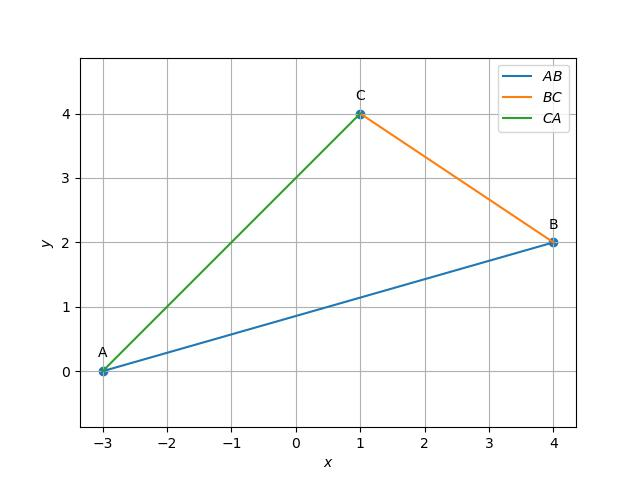
\includegraphics[width=\columnwidth]{/sdcard/Module2/figs/tri.jpg}
\caption{$\vec{A},\vec{B},\vec{C}$ plot}
\label{fig1:Triangle}
\end{figure}



\item The parameteric form of the equation  of $AB$ is 
		\begin{align}
			\vec{x}=\vec{A}+k\vec{m}
		\end{align}
		where
		\begin{align}
\vec{m}=\vec{B}-\vec{A}
		\end{align}
is the direction vector of $AB$.\\
Question 1.1.4 :Find the parametric equation of $AB$,$BC$,$CA$.\\
\solution
The parametric equation for AB is given by
\begin{align}
\vec{x} &= \vec{A} + k\vec{m}\\
\text{where, } \vec{m} &= \vec{B} -\vec{A}\\
&= \myvec{7 \\2}
\end{align}
Hence we get,
\begin{align}
AB: \vec{x} = &\myvec{-3\\0} + k \myvec{7\\2}
\end{align}
Similarly, 
\begin{align}
BC: \vec{x} = &\myvec{4\\2} + k \myvec{-3\\2}\\
CA: \vec{x} = &\myvec{1\\4} + k \myvec{-4\\-4}
\end{align}


\item The normal form of the equation of $AB$  is 
		\begin{align}
			\vec{n}^{\top}\brak{	\vec{x}-\vec{A}} = 0
		\end{align}
		where 
		\begin{align}
			\vec{n}^{\top}\vec{m}&=\vec{n}^{\top}\brak{\vec{B}-\vec{A}} = 0
			\\
			\text{or, } \vec{n}&=\myvec{0 & 1 \\ -1 & 0} \vec{m}
		\end{align}
  \begin{align}
\vec{n}^{\top}\myvec{\vec{x}-\vec{A}}=0
\end{align}
where
\begin{align}
\vec{n}^{\top}\vec{m}&=\vec{n}^{\top}\myvec{\vec{B}-\vec{A}}=0
\end{align}	
or,\begin{align}
\vec{n}&=\myvec{0 &1 \\-1 & 0}\vec{m}
\end{align}
Question 1.1.5:Find the normal form of the equations of $AB, BC$ and $CA$.\\
\solution:
       The normal equation for the side $AB$ is
\begin{align}
\vec{n}^{\top}\myvec{\vec{x}-\vec{A}}&=0\\
\implies
\vec{n}^{\top}\vec{x}&=\vec{n}^{\top}\vec{A}
\end{align}
Now our task is to find the $\vec{n}$ so that we can find $\vec{n}^{\top}$.
As given in the question 
\begin{align}
  \vec{n} &= \myvec{0 & 1\\
  -1 & 0}\vec{m}
\end{align}
Here $\vec{m} = \vec{B}- \vec{A}$ for side $\vec{AB}$
\begin{align}
\implies
\vec{m}&=\myvec{5\\4} - \myvec{1\\0}\\
&=\myvec{4\\4}
\end{align}
Now as we have obtained vector $\vec{m}$.
we can use this to obtain vector $\vec{n}$
\begin{align}
\vec{n} &= \myvec{0 & 1\\
  -1 & 0}\myvec{4\\4}
 = \myvec{4\\-4}
\end{align}
The transpose of $\vec{n}$ is
\begin{align}
  \vec{n}^{\top}&=\myvec{4 & -4}
\end{align}
Hence the normal equation of side $AB$ is 
\begin{align}
    \myvec{4 & -4}\vec{x}&=\myvec{4 & -4}\myvec{1\\0}\\
    \implies
    \myvec{4 & -4}\vec{x}&=4
\end{align}
\begin{figure}
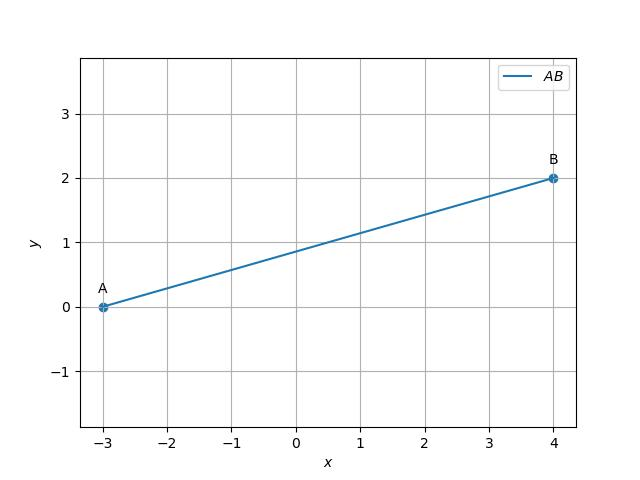
\includegraphics [width=\columnwidth] {/sdcard/Module2/figs/tri1.jpg}
\caption{ The line $\vec{AB}$ plotted using python}
\label{fig: lineab}
\end{figure}


       The normal equation for the side $BC$ is
\begin{align}
\vec{n}^{\top}\myvec{\vec{x}-\vec{B}}&=0\\
\implies
\vec{n}^{\top}\vec{x}&=\vec{n}^{\top}\vec{B}
\end{align}
Now our task is to find the $\vec{n}$ so that we can find $\vec{n}^{\top}$.
As given in the question 
\begin{align}
  \vec{n} &= \myvec{0 & 1\\
  -1 & 0}\vec{m}
\end{align}
Here $\vec{m} = \vec{C}- \vec{B}$ for side $\vec{BC}$
\begin{align}
\implies
\vec{m}&=\myvec{-4\\0} - \myvec{5\\4}\\
&=\myvec{-9\\-4}
\end{align}
Now as we have obtained vector $\vec{m}$.
we can use this to obtain vector $\vec{n}$
\begin{align}
\vec{n} &= \myvec{0 & 1\\
  -1 & 0}\myvec{-9\\-4}
 = \myvec{-4\\9}
\end{align}
The transpose of $\vec{n}$ is
\begin{align}
  \vec{n}^{\top}&=\myvec{-4 & 9}
\end{align}
Hence the normal equation of side $BC$ is 
\begin{align}
    \myvec{-4 & 9}\vec{x}&=\myvec{-4 & 9}\myvec{5\\4}\\
    \implies
    \myvec{-4 & 9}\vec{x}&=16
\end{align}
\begin{figure}
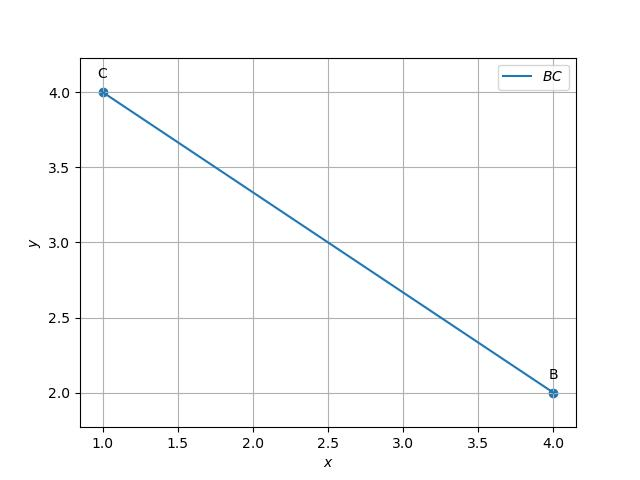
\includegraphics [width=\columnwidth] {/sdcard/Module2/figs/tri2.jpg}
\caption{ The line $\vec{BC}$ plotted using python}
\label{fig: linebc}
\end{figure}



       The normal equation for the side $CA$ is
\begin{align}
\vec{n}^{\top}\myvec{\vec{x}-\vec{C}}&=0\\
\implies
\vec{n}^{\top}\vec{x}&=\vec{n}^{\top}\vec{C}
\end{align}
Now our task is to find the $\vec{n}$ so that we can find $\vec{n}^{\top}$.
As given in the question 
\begin{align}
  \vec{n} &= \myvec{0 & 1\\
  -1 & 0}\vec{m}
\end{align}
Here $\vec{m} = \vec{A}- \vec{C}$ for side $\vec{CA}$
\begin{align}
\implies
\vec{m}&=\myvec{1\\0} - \myvec{-4\\0}\\
&=\myvec{5\\0}
\end{align}
Now as we have obtained vector $\vec{m}$.
we can use this to obtain vector $\vec{n}$
\begin{align}
\vec{n} &= \myvec{0 & 1\\
  -1 & 0}\myvec{5\\0}
 = \myvec{0\\-5}
\end{align}
The transpose of $\vec{n}$ is
\begin{align}
  \vec{n}^{\top}&=\myvec{0 & -5}
\end{align}
Hence the normal equation of side $CA$ is 
\begin{align}
    \myvec{0 & -5}\vec{x}&=\myvec{0 & -5}\myvec{-4\\0}\\
    \implies
    \myvec{0 & -5}\vec{x}&=0
\end{align}
\begin{figure}
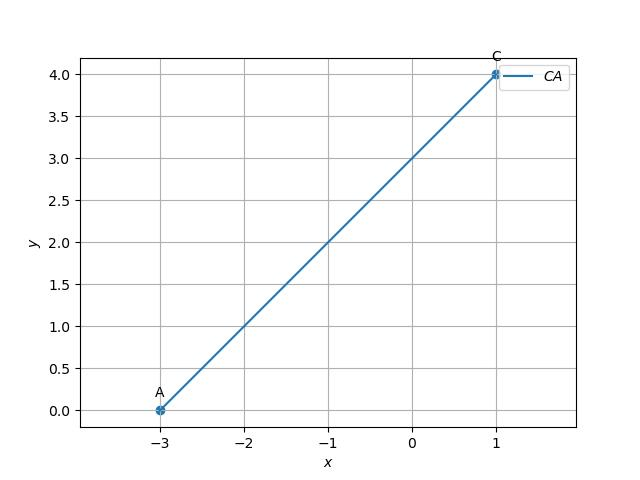
\includegraphics [width=\columnwidth] {/sdcard/Module2/figs/tri3.jpg}
\caption{ The line $\vec{CA}$ plotted using python}
\label{fig: lineca}
\end{figure}


\item The area of $\triangle ABC$ is defined as
		\begin{align}
			\frac{1}{2}\norm{{\brak{\vec{A}-\vec{B}}\times {\vec{A}-\vec{C}}}}
		\end{align}
		where
		\begin{align}
			\vec{A}\times\vec{B} \triangleq \mydet{-3 & 0 \\4 & 2}
		\end{align}
Question 1.1.6:Find the area of $\triangle$ ABC.\\
\solution
Given,
\begin{align}
\vec{A} = \myvec{-3\\0};
\vec{B} = \myvec{4\\2};
\vec{C} = \myvec{1\\4}\\
\vec{A}-\vec{B}=\myvec{-3\\0}-\myvec{4\\2}&=\myvec{-7\\-2}\\
\vec{A}-\vec{C}=\myvec{-3\\0}-\myvec{1\\4}&=\myvec{-4\\-4}\\
\therefore(\vec{A}-\vec{B})\times(\vec{A}-\vec{C}) &=\mydet{-7 & -2\\-4 & -4}\\&=20\\
\implies\frac{1}{2}\norm{(\vec{A}-\vec{B})\times(\vec{A}-\vec{C})}&=\frac{20}{2}=10
\end{align}


\item
Question 1.1.7:Find the angles $\vec{A},\vec{B},\vec{C}$, given that 
\begin{align}
	\cos{A} \triangleq \frac{(\vec{B}-\vec{A})\top(\vec{C}-\vec{A})}{\norm{\vec{B}-\vec{A}}\norm{\vec{C}-\vec{A}}}
\end{align}
\solution 
\\
From the given values of $\vec{A},\vec{B},\vec{C}$,\\
\begin{enumerate}

\item Finding the value of angle A
\begin{align}
	\vec{B}-\vec{A} &=\myvec{7\\2}
\end{align}
and 
\begin{align}
	\vec{C}-\vec{A}&= \myvec{4\\4}
\end{align}
also calculating the values of norms
\begin{align}
	\norm{\vec{B}-\vec{A}} &= \sqrt{53} \\
	\norm{\vec{C}-\vec{A}} &= \sqrt{32} 
\end{align}
and by doing matrix multiplication we get,
\begin{align}
\begin{split}
	(\vec{B}-\vec{A})^{\top}(\vec{C}-\vec{A})&=\myvec{7&2}\myvec{4\\4}\\
	&=36
\end{split}
\end{align}
so 
\begin{align}
	\cos{A}&= \frac{36}{\sqrt{53} \sqrt{32}}
	\implies A&=\cos^{-1}{ \frac{36}{\sqrt{53} \sqrt{32}}}
\end{align}




\item Finding the value of angle B
\begin{align}
	\vec{C}-\vec{B} &=\myvec{-3\\2}
\end{align}
and 
\begin{align}
	\vec{A}-\vec{B}&= \myvec{-7\\-2}
\end{align}
also calculating the values of norms
\begin{align}
	\norm{\vec{C}-\vec{B}} &= \sqrt{53}\\
	\norm{\vec{A}-\vec{B}} &= \sqrt{13}
\end{align}
and by doing matrix multiplication we get,
\begin{align}
\begin{split}
	(\vec{C}-\vec{B})^{\top}(\vec{A}-\vec{B})&=\myvec{-3&2}\myvec{-7\\-2}\\
	&= 17
\end{split}
\end{align}
so 
\begin{align}
	\cos{B}&= \frac{17}{\sqrt{53} \sqrt{13}}
	\implies B&=\cos^{-1}{ \frac{17}{\sqrt{53} \sqrt{13}}}
\end{align}



\item Finding the value of angle C
\begin{align}
	\vec{A}-\vec{C} &=\myvec{-4\\-4}
\end{align}
and 
\begin{align}
	\vec{B}-\vec{C}&= \myvec{3\\2}
\end{align}
also calculating the values of norms
\begin{align}
	\norm{\vec{A}-\vec{C}} &= \sqrt{32}\\
	\norm{\vec{B}-\vec{C}} &= \sqrt{13}
\end{align}
and by doing matrix multiplication we get,
\begin{align}
\begin{split}
	(\vec{A}-\vec{C})^{\top}(\vec{B}-\vec{C})&=\myvec{-4&-4}\myvec{3\\2}\\
	&=-20
\end{split}
\end{align}
so 
\begin{align}
	\cos{C}&= \frac{-20}{\sqrt{32} \sqrt{13}}
	\implies C&=\cos^{-1}{ \frac{-20}{\sqrt{32} \sqrt{13}}}
\end{align}
\end{enumerate}
\end{enumerate}
%\section{Median}
%\documentclass[11pt]{book}
\usepackage{gvv-book}
\usepackage{gvv}
\usepackage[sectionbib,authoryear]{natbib}
\setcounter{secnumdepth}{3}
\setcounter{tocdepth}{2}
\makeindex

\begin{document}
\frontmatter
\tableofcontents
\setcounter{page}{1}
\mainmatter
\chapter{Triangle}
Consider a triangle with vertices
\begin{align}
\label{eq:tri-pts}
\vec{A}=\myvec{1 \\ 0},\,
\vec{B}=\myvec{5\\4},\,
	\vec{c}=\myvec{-4\\0},\,
\end{align}

\section{Vectors}
\section{median}


\begin{enumerate}[label=\thesection.\arabic*.,ref=\thesection.\theenumi]
\numberwithin{equation}{enumi}

%Question 1.2.1:
\item  If $\vec{D}$ divides $BC$ in the ratio $k : 1$,
		\begin{align}
			\vec{D}= \frac{k\vec{C}+\vec{B}}{k+1}
		\end{align}
Find the mid points $\vec{D}, \vec{E}, \vec{F}$ of the sides $BC, CA$ and $AB$ respectively.\\
If $\vec{D}$ divides $BC$ in the ratio $k : 1$,
\begin{align}
\vec{D}= \frac{k\vec{C}+\vec{B}}{k+1}
\end{align}
Find the mid points $\vec{D}, \vec{E}, \vec{F}$ of the sides $BC, CA$ and $AB$ respectively.
\newline
Given:
\begin{align}
\vec{A} &= \myvec{-3\\0\\}\\
\vec{B} &= \myvec{4\\2\\}\\
\vec{C} &= \myvec{1\\4\\}
\end{align}

\solution
Since $\vec{D}$ is the midpoint of $BC$,
\begin{align}
k &= 1\\
\implies \vec{D} &= \frac{\vec{C} + \vec{B}}{2}\\
&= \frac{1}{2}\myvec{5\\6}
\end{align}
Similarly,
\begin{align}
\vec{E} &= \frac{\vec{A} + \vec{C}}{2}\\
&= \frac{1}{2}\myvec{-2\\4}\\
\vec{F} &= \frac{\vec{A} + \vec{B}}{2}\\
&= \myvec{1/2\\1}
\end{align} 

%Question 1.2.2:
\item Find the equations of $AD, BE$ and $CF$.\\
\\ \solution:
$\vec{D}$,$\vec{E}$,$\vec{F}$ are the midpoints of $BC$,$CA$,$AB$ respectively, then\\
\begin{align}
 \vec{D} &=  \myvec{\frac{5}{2}\\3}\\
 \vec{E} &=  \myvec{-1\\2}\\
 \vec{F} &= \myvec{1/2\\1}
\end{align}
\begin{enumerate}

 \item The normal equation for the median $AD$ is
  \begin{align}
    \vec{n}^{\top}\myvec{\vec{x}-\vec{A}}&=0\\
    \implies
    \vec{n}^{\top}\vec{x}&=\vec{n}^{\top}\vec{A}
  \end{align}
 We have to find the $\vec{n}$ so that we can find $\vec{n}^{\top}$.
 Since,
\begin{align}
  \vec{n} &= \myvec{0 & 1\\
  -1 & 0}\vec{m}
\end{align}
Here $\vec{m} = \vec{D}- \vec{A}$ for median $AD$
\begin{align}
\vec{m}&=\myvec{\frac{11}{2}\\3}
\end{align}
Since,
\begin{align}
  \vec{n} &= \myvec{0 & 1\\
  -1 & 0}\vec{m}\\
\implies
\vec{n} &= \myvec{0 & 1\\
  -1 & 0}\myvec{\frac{11}{2}\\3}\\
        &= \myvec{3 \\\frac{-11}{2}}
\end{align}
Hence the normal equation of median $AD$ is 
\begin{align}
    \myvec{3 & \frac{-11}{2}}\vec{x}&=\myvec{3 & \frac{-11}{2}}\myvec{-3\\0}\\
    \implies
    \myvec{3 & \frac{-11}{2}}\vec{x}&={-9}
\end{align}

\item The normal equation for the median $BE$ is
\begin{align}
\vec{n}^{\top}\myvec{\vec{x}-\vec{B}}&=0\\
\implies
\vec{n}^{\top}\vec{x}&=\vec{n}^{\top}\vec{B}
\end{align}
Here $\vec{m} = \vec{E}- \vec{B}$ for median $BE$
\begin{align}
\vec{m}&&=\myvec{-5\\0}
\end{align}
Since,
\begin{align}
  \vec{n} &= \myvec{0 & 1\\
  -1 & 0}\vec{m}\\
\implies
\vec{n} &= \myvec{0 & 1\\
  -1 & 0}\myvec{-5\\0}\\
        &= \myvec{0\\ 5}
\end{align}
Hence the normal equation of median $BE$ is 
\begin{align}
    \myvec{0 & 5}\vec{x}&=\myvec{0 & 5}\myvec{4\\2}\\
\implies
    \myvec{0 & 5}\vec{x}&={10}
\end{align}

\item The normal equation for the median $CF$ is
\begin{align}
\vec{n}^{\top}\myvec{\vec{x}-\vec{C}}&=0\\
\implies
\vec{n}^{\top}\vec{x}&=\vec{n}^{\top}\vec{C}
\end{align}
Here $\vec{m} = \vec{F}- \vec{C}$ for median $CF$
\begin{align}
\vec{m}&=\myvec{\frac{-1}{2}\\-3}
\end{align}
Since,
\begin{align}
  \vec{n} &= \myvec{0 & 1\\
  -1 & 0}\vec{m}\\
\implies
\vec{n} &= \myvec{0 & 1\\
  -1 & 0}\myvec{\frac{-1}{2} \\ -3 }\\
        &= \myvec{-3 \\ \frac{1}{2}}
\end{align}
Hence the normal equation of median $CF$ is 
\begin{align}
    \myvec{-3 & \frac{1}{2} }\vec{x}&=\myvec{-3 & \frac{1}{2}}\myvec{1\\4}\\
\implies
    \myvec{-3 & \frac{1}{2}}\vec{x}&=-1
\end{align}
\end{enumerate}

%Question 1.2.3:
\item Find the intersection $\vec{G}$ of $BE$ and $CF$
\\ 
\solution 
$\vec{A},\vec{B}$ and $\vec{C}$ are vertices of triangle:
\begin{align}
    \vec{A} &= \myvec-3 \\0} \\
    \vec{B} &= \myvec{4\\ 2} \\
    \vec{C} &= \myvec{1 \\4}
\end{align}
Since $\vec{E}$ and $\vec{F}$ are midpoints of $CA$ and $AB$,
\begin{align}
    \vec{E} &= \frac{\vec{A} + \vec{C}}{2} \\
	&= \myvec{-1 \\2}\\
    \vec{F} &= \frac{\vec{B} + \vec{A}}{2} \\ 
    &= \myvec{ \frac{1}{2} \\ 1}
\end{align}
The line $BE$ in vector form is given by
\begin{align}
\myvec{0 & 5} \vec{x} &= \myvec{10}
\label{eq:1.2.3,8}
\end{align}
The line $CF$ in vector form is given by
\begin{align}
\myvec{ -3&-\frac{1}{2}} \vec{x} &= \myvec{-1}
\label{eq:1.2.3,9}
\end{align}
From \eqref{eq:1.2.3,8} and \eqref{eq:1.2.3,9} the augmented matrix is:
\begin{align}
\myvec{
0 & 5 & {10} \\
-3 & \frac{1}{2} & -1
}
\end{align}
Solve for $\vec{x}$ using Gauss-Elimination method:
\begin{align}
    \label{eq:matrowoperations}
    \myvec{
    1 & 0 & \frac{2}{3}
    \\
    0 & 1 & 2
    }
\end{align} 
Therefore, 
\begin{align}
\vec{G} = \myvec{\frac{2}{3} \\ 2}
\end{align}
From Fig. \ref{fig:Triangle101}, We can see that $\vec{G}=\myvec{\frac{2}{3}\\ 2}$ is the intersection of $BE$ and $CF$
\begin{figure}[h]
\centering
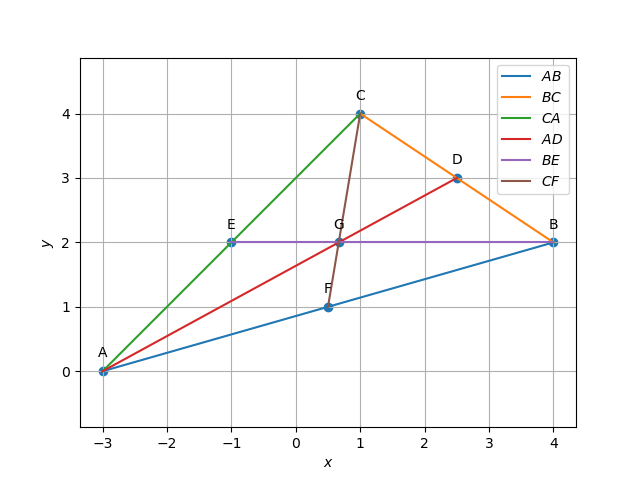
\includegraphics[width=\columnwidth]{/sdcard/geometry/geometry/figs/med2.png}
\caption{$G$ is the centroid of triangle $ABC$}
\label{fig:Triangle101}
\end{figure}



%Question 1.2.4:
\item Verify that 
		\begin{align}
			\frac{BG}{GE} = 
			\frac{CG}{GF} =
			\frac{AG}{GD} =2 
		\end{align}\\
Question 1.2.4:Verify that 
\begin{align}
		\frac{BG}{GE} = 
		\frac{CG}{GF} =
		\frac{AG}{GD} = 2 
\end{align}
\solution In order to verify the above equation we first need to find $\vec{G}$.$\vec{G}$ is the intersection of $BE$ and $CF$,Using the value of $\vec{G}$ from (1.2.3).
\begin{align}
		\vec{G} = \myvec{\frac{2}{3}\\2}
\end{align}
Also,We know that $\vec{D}, \vec{E}$ and $\vec{F}$ are midpoints of $BC, CA$ and $AB$ respectively from (1.2.1).
\begin{align}
		\vec{D} = \myvec{\frac{5}{2} \\ 3},\,
		\vec{E} = \myvec{-1 \\ 2},\,
		\vec{F} = \myvec{\frac{1}{2}\\ 1}
\end{align}
\begin{enumerate}
\item Calculating the ratio of $BG$ and $GE$,
\begin{align}
		\label{eq:tri-pts/4} \vec{G}-\vec{B} &= \myvec{\frac{-10}{3} \\ 0} \\
		\label{eq:tri-pts/5} \vec{E}-\vec{G} &= \myvec{\frac{-5}{3} \\ 0} \\
		\label{eq:tri-pts/6} \norm{\vec{G}-\vec{B}} &= \sqrt{\brak{\frac{-10}{0}}^2 + \brak{\frac{-5}{0}}^{2}}  \\
		\label{eq:tri-pts/7} \norm{\vec{E}-\vec{G}} &= \sqrt{\brak{\frac{-13}{6}}^2 + \brak{\frac{-4}{3}}^2} &= \frac{\sqrt{233}}{6} \\
		\label{eq:tri-pts/8}\frac{BG}{GE} &= \frac{\norm{\vec{G}-\vec{B}}}{\norm{\vec{E}-\vec{G}}}&= 2  
\end{align}		
\end{enumerate}

From \eqref{eq:tri-pts/8}, \eqref{eq:tri-pts/13}, \eqref{eq:tri-pts/18}
\begin{align}
		\frac{BG}{GE} = 
		\frac{CG}{GF} =
		\frac{AG}{GD} = 2
\end{align}
Hence verified.



%Question 1.2.5:
\item Show that $\vec{A}, \vec{G}$ and $\vec{D}$ are collinear.\\
\solution 
Given that,
\begin{align}
    \vec{A} = \myvec{-3\\0}
    \quad
    \vec{B} &= \myvec{4\\2}
    \quad
    \vec{C} = \myvec{1\\4}
\end{align}
We need to show that points $\vec{A},\vec{D},\vec{G}$ are collinear.
From Problem 1.2.3 We know that, The point $\vec{G}$ is 
\begin{align}
    \vec{G} &=\myvec{\frac{2}{3}\\ 2}
\end{align}
And from Problem 1.2.1 We know that, The point $\vec{D}$ is 
\begin{align}
    \vec{D} &=\myvec{\frac{5}{2}\\ 3}
\end{align}
In Problem 1.1.3, There is a theorem/law mentioned i.e.,

Points $\vec{A},\vec{D},\vec{G}$ are defined to be collinear if 
\begin{align}
    \text{rank}\myvec{
    1 & 1 & 1\\
    \vec{A} & \vec{D} & \vec{G} \\
    } &= 2 
\end{align} 
Using the above law/Theorem Let
\begin{align}
    \vec{R}&=\myvec{
    1 & 1 & 1
    \\
    -3 & \frac{5}{2} & \frac{2}{3}
    \\
    0 & 3 & 2
    } 
\end{align} 
The matrix $\vec{R}$ can be row reduced as follows,
\begin{align}
    \label{eq:mat_row_operations}
    \myvec{
    1 & 1 & 1
    \\
    -3 & \frac{5}{2} & \frac{2}{3}
    \\
    0 & 3 & 2
    }
     \xleftrightarrow[]{}
    \myvec{
    1 & 1 & 1
    \\
    0 & 1 & \frac{2}{3}
    \\
    0 & 0 & 0
    }
\end{align}
Rank of above matrix is 2.\\
Hence, we proved that that points $\vec{A},\vec{D},\vec{G}$ are collinear.



%Question 1.2.6:
\item Verify that 
		\begin{align}
			\vec{G}=\frac{\vec{A}+\vec{B}+\vec{C}}{3}
		\end{align}
$\vec{G}$ is known as the {\em centroid} of $\triangle ABC$.\\
Verify that\\
\begin{align}
 \vec{G}=\frac{\vec{A}+\vec{B}+\vec{C}}{3}   
\end{align}
$\vec{G}$ is known as the \underline{centroid} of $\triangle$ABC 
SOLUTION:\\
let us first evaluate the R.H.S of the equation
\begin{equation}
\begin{split}
\label{eq:centroid}
    \vec{G}&= \frac{\myvec{-3\\0}+\myvec{4\\2}+\myvec{1\\4}}{3}\\   
     &= \myvec{\frac{2}{3}\\ 2}
\end{split}
\end{equation}
Hence verified.


%Question 1.2.7: 
\item Verify that 
		\begin{align}
\vec{A}-\vec{F}=\vec{E}-\vec{D}
		\end{align}
The quadrilateral $AFDE$ is defined to be a parallelogram.\\
Question : Verify that 
\begin{align}
	\vec{A}-\vec{F} = \vec{E}-\vec{D}
\end{align}
The quadrilateral $AFDE$ is defined to be parallelogram
\\ \solution 
Given that,
\begin{align}
    \vec{A} = \myvec{-3\\0}
    \quad
    \vec{B} &= \myvec{4\\2}
    \quad
    \vec{C} = \myvec{1\\4}
\end{align}
From Problem 1.2.1 We know that, The point $\vec{D},\vec{E},\vec{F}$ is 
\begin{align}
    \vec{D} = \myvec{\frac{5}{2}\\ 3 }
    \quad
    \vec{E} &= \myvec{-1\\2}
    \quad
    \vec{F} = \myvec{\frac{1}{2}\\ 1}
\end{align}
Evaluating the R.H.S of the equation
\begin{align}
    \vec{A}-\vec{F}&=\myvec{ \frac{-7}{2} \\ -1 }
\end{align} 
Evaluating the L.H.S of the equation
\begin{align}
    \vec{E}-\vec{D}&=\myvec{\frac{-7}{2} \\ -1 }
\end{align}
Hence verified that, R.H.S = L.H.S i.e.,
\begin{align}
	\vec{A}-\vec{F} = \vec{E}-\vec{D}
\end{align}
From the fig\ref{fig:Triangle}, It is verified that $AFDE$ is a parallelogram
\begin{figure}
\centering
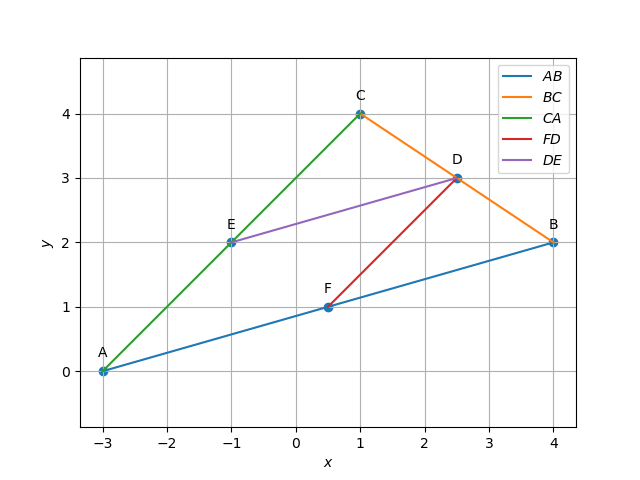
\includegraphics[width=\columnwidth]{/sdcard/geometry/geometry/figs/prm.png}
\caption{$AFDE$ form a parallelogram in triangle ABC}
\label{fig:Triangle}
\end{figure}
\end{enumerate}














%\documentclass[11pt]{book}
\usepackage{gvv-book}
\usepackage{gvv}
\usepackage[sectionbib,authoryear]{natbib}
\setcounter{secnumdepth}{3}
\setcounter{tocdepth}{2}
\makeindex

\begin{document}
\frontmatter
\tableofcontents
\setcounter{page}{1}
\mainmatter
\chapter{Triangle}
Consider a triangle with vertices
\begin{align}
\label{eq:tri-pts}
\vec{A}=\myvec{1 \\ 0},\,
\vec{B}=\myvec{5\\4},\,
	\vec{c}=\myvec{-4\\0},\,
\end{align}

\section{Vectors}
\section{median}


\begin{enumerate}[label=\thesection.\arabic*.,ref=\thesection.\theenumi]
\numberwithin{equation}{enumi}

%Question 1.2.1:
\item  If $\vec{D}$ divides $BC$ in the ratio $k : 1$,
		\begin{align}
			\vec{D}= \frac{k\vec{C}+\vec{B}}{k+1}
		\end{align}
Find the mid points $\vec{D}, \vec{E}, \vec{F}$ of the sides $BC, CA$ and $AB$ respectively.\\
If $\vec{D}$ divides $BC$ in the ratio $k : 1$,
\begin{align}
\vec{D}= \frac{k\vec{C}+\vec{B}}{k+1}
\end{align}
Find the mid points $\vec{D}, \vec{E}, \vec{F}$ of the sides $BC, CA$ and $AB$ respectively.
\newline
Given:
\begin{align}
\vec{A} &= \myvec{-3\\0\\}\\
\vec{B} &= \myvec{4\\2\\}\\
\vec{C} &= \myvec{1\\4\\}
\end{align}

\solution
Since $\vec{D}$ is the midpoint of $BC$,
\begin{align}
k &= 1\\
\implies \vec{D} &= \frac{\vec{C} + \vec{B}}{2}\\
&= \frac{1}{2}\myvec{5\\6}
\end{align}
Similarly,
\begin{align}
\vec{E} &= \frac{\vec{A} + \vec{C}}{2}\\
&= \frac{1}{2}\myvec{-2\\4}\\
\vec{F} &= \frac{\vec{A} + \vec{B}}{2}\\
&= \myvec{1/2\\1}
\end{align} 

%Question 1.2.2:
\item Find the equations of $AD, BE$ and $CF$.\\
\\ \solution:
$\vec{D}$,$\vec{E}$,$\vec{F}$ are the midpoints of $BC$,$CA$,$AB$ respectively, then\\
\begin{align}
 \vec{D} &=  \myvec{\frac{5}{2}\\3}\\
 \vec{E} &=  \myvec{-1\\2}\\
 \vec{F} &= \myvec{1/2\\1}
\end{align}
\begin{enumerate}

 \item The normal equation for the median $AD$ is
  \begin{align}
    \vec{n}^{\top}\myvec{\vec{x}-\vec{A}}&=0\\
    \implies
    \vec{n}^{\top}\vec{x}&=\vec{n}^{\top}\vec{A}
  \end{align}
 We have to find the $\vec{n}$ so that we can find $\vec{n}^{\top}$.
 Since,
\begin{align}
  \vec{n} &= \myvec{0 & 1\\
  -1 & 0}\vec{m}
\end{align}
Here $\vec{m} = \vec{D}- \vec{A}$ for median $AD$
\begin{align}
\vec{m}&=\myvec{\frac{11}{2}\\3}
\end{align}
Since,
\begin{align}
  \vec{n} &= \myvec{0 & 1\\
  -1 & 0}\vec{m}\\
\implies
\vec{n} &= \myvec{0 & 1\\
  -1 & 0}\myvec{\frac{11}{2}\\3}\\
        &= \myvec{3 \\\frac{-11}{2}}
\end{align}
Hence the normal equation of median $AD$ is 
\begin{align}
    \myvec{3 & \frac{-11}{2}}\vec{x}&=\myvec{3 & \frac{-11}{2}}\myvec{-3\\0}\\
    \implies
    \myvec{3 & \frac{-11}{2}}\vec{x}&={-9}
\end{align}

\item The normal equation for the median $BE$ is
\begin{align}
\vec{n}^{\top}\myvec{\vec{x}-\vec{B}}&=0\\
\implies
\vec{n}^{\top}\vec{x}&=\vec{n}^{\top}\vec{B}
\end{align}
Here $\vec{m} = \vec{E}- \vec{B}$ for median $BE$
\begin{align}
\vec{m}&&=\myvec{-5\\0}
\end{align}
Since,
\begin{align}
  \vec{n} &= \myvec{0 & 1\\
  -1 & 0}\vec{m}\\
\implies
\vec{n} &= \myvec{0 & 1\\
  -1 & 0}\myvec{-5\\0}\\
        &= \myvec{0\\ 5}
\end{align}
Hence the normal equation of median $BE$ is 
\begin{align}
    \myvec{0 & 5}\vec{x}&=\myvec{0 & 5}\myvec{4\\2}\\
\implies
    \myvec{0 & 5}\vec{x}&={10}
\end{align}

\item The normal equation for the median $CF$ is
\begin{align}
\vec{n}^{\top}\myvec{\vec{x}-\vec{C}}&=0\\
\implies
\vec{n}^{\top}\vec{x}&=\vec{n}^{\top}\vec{C}
\end{align}
Here $\vec{m} = \vec{F}- \vec{C}$ for median $CF$
\begin{align}
\vec{m}&=\myvec{\frac{-1}{2}\\-3}
\end{align}
Since,
\begin{align}
  \vec{n} &= \myvec{0 & 1\\
  -1 & 0}\vec{m}\\
\implies
\vec{n} &= \myvec{0 & 1\\
  -1 & 0}\myvec{\frac{-1}{2} \\ -3 }\\
        &= \myvec{-3 \\ \frac{1}{2}}
\end{align}
Hence the normal equation of median $CF$ is 
\begin{align}
    \myvec{-3 & \frac{1}{2} }\vec{x}&=\myvec{-3 & \frac{1}{2}}\myvec{1\\4}\\
\implies
    \myvec{-3 & \frac{1}{2}}\vec{x}&=-1
\end{align}
\end{enumerate}

%Question 1.2.3:
\item Find the intersection $\vec{G}$ of $BE$ and $CF$
\\ 
\solution 
$\vec{A},\vec{B}$ and $\vec{C}$ are vertices of triangle:
\begin{align}
    \vec{A} &= \myvec-3 \\0} \\
    \vec{B} &= \myvec{4\\ 2} \\
    \vec{C} &= \myvec{1 \\4}
\end{align}
Since $\vec{E}$ and $\vec{F}$ are midpoints of $CA$ and $AB$,
\begin{align}
    \vec{E} &= \frac{\vec{A} + \vec{C}}{2} \\
	&= \myvec{-1 \\2}\\
    \vec{F} &= \frac{\vec{B} + \vec{A}}{2} \\ 
    &= \myvec{ \frac{1}{2} \\ 1}
\end{align}
The line $BE$ in vector form is given by
\begin{align}
\myvec{0 & 5} \vec{x} &= \myvec{10}
\label{eq:1.2.3,8}
\end{align}
The line $CF$ in vector form is given by
\begin{align}
\myvec{ -3&-\frac{1}{2}} \vec{x} &= \myvec{-1}
\label{eq:1.2.3,9}
\end{align}
From \eqref{eq:1.2.3,8} and \eqref{eq:1.2.3,9} the augmented matrix is:
\begin{align}
\myvec{
0 & 5 & {10} \\
-3 & \frac{1}{2} & -1
}
\end{align}
Solve for $\vec{x}$ using Gauss-Elimination method:
\begin{align}
    \label{eq:matrowoperations}
    \myvec{
    1 & 0 & \frac{2}{3}
    \\
    0 & 1 & 2
    }
\end{align} 
Therefore, 
\begin{align}
\vec{G} = \myvec{\frac{2}{3} \\ 2}
\end{align}
From Fig. \ref{fig:Triangle101}, We can see that $\vec{G}=\myvec{\frac{2}{3}\\ 2}$ is the intersection of $BE$ and $CF$
\begin{figure}[h]
\centering
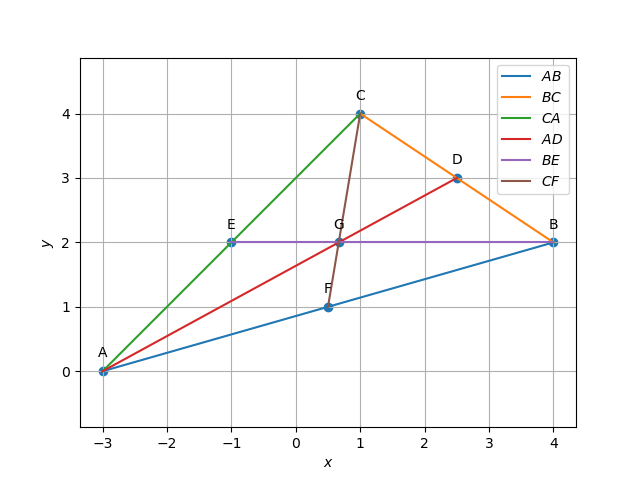
\includegraphics[width=\columnwidth]{/sdcard/geometry/geometry/figs/med2.png}
\caption{$G$ is the centroid of triangle $ABC$}
\label{fig:Triangle101}
\end{figure}



%Question 1.2.4:
\item Verify that 
		\begin{align}
			\frac{BG}{GE} = 
			\frac{CG}{GF} =
			\frac{AG}{GD} =2 
		\end{align}\\
Question 1.2.4:Verify that 
\begin{align}
		\frac{BG}{GE} = 
		\frac{CG}{GF} =
		\frac{AG}{GD} = 2 
\end{align}
\solution In order to verify the above equation we first need to find $\vec{G}$.$\vec{G}$ is the intersection of $BE$ and $CF$,Using the value of $\vec{G}$ from (1.2.3).
\begin{align}
		\vec{G} = \myvec{\frac{2}{3}\\2}
\end{align}
Also,We know that $\vec{D}, \vec{E}$ and $\vec{F}$ are midpoints of $BC, CA$ and $AB$ respectively from (1.2.1).
\begin{align}
		\vec{D} = \myvec{\frac{5}{2} \\ 3},\,
		\vec{E} = \myvec{-1 \\ 2},\,
		\vec{F} = \myvec{\frac{1}{2}\\ 1}
\end{align}
\begin{enumerate}
\item Calculating the ratio of $BG$ and $GE$,
\begin{align}
		\label{eq:tri-pts/4} \vec{G}-\vec{B} &= \myvec{\frac{-10}{3} \\ 0} \\
		\label{eq:tri-pts/5} \vec{E}-\vec{G} &= \myvec{\frac{-5}{3} \\ 0} \\
		\label{eq:tri-pts/6} \norm{\vec{G}-\vec{B}} &= \sqrt{\brak{\frac{-10}{0}}^2 + \brak{\frac{-5}{0}}^{2}}  \\
		\label{eq:tri-pts/7} \norm{\vec{E}-\vec{G}} &= \sqrt{\brak{\frac{-13}{6}}^2 + \brak{\frac{-4}{3}}^2} &= \frac{\sqrt{233}}{6} \\
		\label{eq:tri-pts/8}\frac{BG}{GE} &= \frac{\norm{\vec{G}-\vec{B}}}{\norm{\vec{E}-\vec{G}}}&= 2  
\end{align}		
\end{enumerate}

From \eqref{eq:tri-pts/8}, \eqref{eq:tri-pts/13}, \eqref{eq:tri-pts/18}
\begin{align}
		\frac{BG}{GE} = 
		\frac{CG}{GF} =
		\frac{AG}{GD} = 2
\end{align}
Hence verified.



%Question 1.2.5:
\item Show that $\vec{A}, \vec{G}$ and $\vec{D}$ are collinear.\\
\solution 
Given that,
\begin{align}
    \vec{A} = \myvec{-3\\0}
    \quad
    \vec{B} &= \myvec{4\\2}
    \quad
    \vec{C} = \myvec{1\\4}
\end{align}
We need to show that points $\vec{A},\vec{D},\vec{G}$ are collinear.
From Problem 1.2.3 We know that, The point $\vec{G}$ is 
\begin{align}
    \vec{G} &=\myvec{\frac{2}{3}\\ 2}
\end{align}
And from Problem 1.2.1 We know that, The point $\vec{D}$ is 
\begin{align}
    \vec{D} &=\myvec{\frac{5}{2}\\ 3}
\end{align}
In Problem 1.1.3, There is a theorem/law mentioned i.e.,

Points $\vec{A},\vec{D},\vec{G}$ are defined to be collinear if 
\begin{align}
    \text{rank}\myvec{
    1 & 1 & 1\\
    \vec{A} & \vec{D} & \vec{G} \\
    } &= 2 
\end{align} 
Using the above law/Theorem Let
\begin{align}
    \vec{R}&=\myvec{
    1 & 1 & 1
    \\
    -3 & \frac{5}{2} & \frac{2}{3}
    \\
    0 & 3 & 2
    } 
\end{align} 
The matrix $\vec{R}$ can be row reduced as follows,
\begin{align}
    \label{eq:mat_row_operations}
    \myvec{
    1 & 1 & 1
    \\
    -3 & \frac{5}{2} & \frac{2}{3}
    \\
    0 & 3 & 2
    }
     \xleftrightarrow[]{}
    \myvec{
    1 & 1 & 1
    \\
    0 & 1 & \frac{2}{3}
    \\
    0 & 0 & 0
    }
\end{align}
Rank of above matrix is 2.\\
Hence, we proved that that points $\vec{A},\vec{D},\vec{G}$ are collinear.



%Question 1.2.6:
\item Verify that 
		\begin{align}
			\vec{G}=\frac{\vec{A}+\vec{B}+\vec{C}}{3}
		\end{align}
$\vec{G}$ is known as the {\em centroid} of $\triangle ABC$.\\
Verify that\\
\begin{align}
 \vec{G}=\frac{\vec{A}+\vec{B}+\vec{C}}{3}   
\end{align}
$\vec{G}$ is known as the \underline{centroid} of $\triangle$ABC 
SOLUTION:\\
let us first evaluate the R.H.S of the equation
\begin{equation}
\begin{split}
\label{eq:centroid}
    \vec{G}&= \frac{\myvec{-3\\0}+\myvec{4\\2}+\myvec{1\\4}}{3}\\   
     &= \myvec{\frac{2}{3}\\ 2}
\end{split}
\end{equation}
Hence verified.


%Question 1.2.7: 
\item Verify that 
		\begin{align}
\vec{A}-\vec{F}=\vec{E}-\vec{D}
		\end{align}
The quadrilateral $AFDE$ is defined to be a parallelogram.\\
Question : Verify that 
\begin{align}
	\vec{A}-\vec{F} = \vec{E}-\vec{D}
\end{align}
The quadrilateral $AFDE$ is defined to be parallelogram
\\ \solution 
Given that,
\begin{align}
    \vec{A} = \myvec{-3\\0}
    \quad
    \vec{B} &= \myvec{4\\2}
    \quad
    \vec{C} = \myvec{1\\4}
\end{align}
From Problem 1.2.1 We know that, The point $\vec{D},\vec{E},\vec{F}$ is 
\begin{align}
    \vec{D} = \myvec{\frac{5}{2}\\ 3 }
    \quad
    \vec{E} &= \myvec{-1\\2}
    \quad
    \vec{F} = \myvec{\frac{1}{2}\\ 1}
\end{align}
Evaluating the R.H.S of the equation
\begin{align}
    \vec{A}-\vec{F}&=\myvec{ \frac{-7}{2} \\ -1 }
\end{align} 
Evaluating the L.H.S of the equation
\begin{align}
    \vec{E}-\vec{D}&=\myvec{\frac{-7}{2} \\ -1 }
\end{align}
Hence verified that, R.H.S = L.H.S i.e.,
\begin{align}
	\vec{A}-\vec{F} = \vec{E}-\vec{D}
\end{align}
From the fig\ref{fig:Triangle}, It is verified that $AFDE$ is a parallelogram
\begin{figure}
\centering
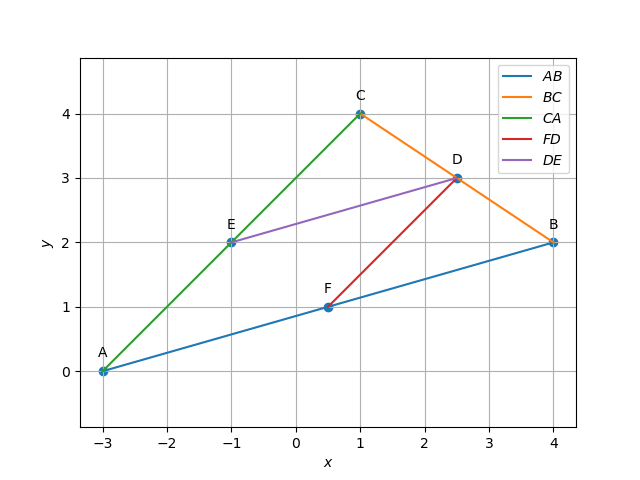
\includegraphics[width=\columnwidth]{/sdcard/geometry/geometry/figs/prm.png}
\caption{$AFDE$ form a parallelogram in triangle ABC}
\label{fig:Triangle}
\end{figure}
\end{enumerate}














%\documentclass[11pt]{book}
\usepackage{gvv-book}
\usepackage{gvv}
\usepackage[sectionbib,authoryear]{natbib}
\setcounter{secnumdepth}{3}
\setcounter{tocdepth}{2}
\makeindex

\begin{document}
\frontmatter
\tableofcontents
\setcounter{page}{1}
\mainmatter
\chapter{Triangle}
Consider a triangle with vertices
\begin{align}
\label{eq:tri-pts}
\vec{A}=\myvec{1 \\ 0},\,
\vec{B}=\myvec{5\\4},\,
	\vec{c}=\myvec{-4\\0},\,
\end{align}

\section{Vectors}
\section{median}


\begin{enumerate}[label=\thesection.\arabic*.,ref=\thesection.\theenumi]
\numberwithin{equation}{enumi}

%Question 1.2.1:
\item  If $\vec{D}$ divides $BC$ in the ratio $k : 1$,
		\begin{align}
			\vec{D}= \frac{k\vec{C}+\vec{B}}{k+1}
		\end{align}
Find the mid points $\vec{D}, \vec{E}, \vec{F}$ of the sides $BC, CA$ and $AB$ respectively.\\
If $\vec{D}$ divides $BC$ in the ratio $k : 1$,
\begin{align}
\vec{D}= \frac{k\vec{C}+\vec{B}}{k+1}
\end{align}
Find the mid points $\vec{D}, \vec{E}, \vec{F}$ of the sides $BC, CA$ and $AB$ respectively.
\newline
Given:
\begin{align}
\vec{A} &= \myvec{-3\\0\\}\\
\vec{B} &= \myvec{4\\2\\}\\
\vec{C} &= \myvec{1\\4\\}
\end{align}

\solution
Since $\vec{D}$ is the midpoint of $BC$,
\begin{align}
k &= 1\\
\implies \vec{D} &= \frac{\vec{C} + \vec{B}}{2}\\
&= \frac{1}{2}\myvec{5\\6}
\end{align}
Similarly,
\begin{align}
\vec{E} &= \frac{\vec{A} + \vec{C}}{2}\\
&= \frac{1}{2}\myvec{-2\\4}\\
\vec{F} &= \frac{\vec{A} + \vec{B}}{2}\\
&= \myvec{1/2\\1}
\end{align} 

%Question 1.2.2:
\item Find the equations of $AD, BE$ and $CF$.\\
\\ \solution:
$\vec{D}$,$\vec{E}$,$\vec{F}$ are the midpoints of $BC$,$CA$,$AB$ respectively, then\\
\begin{align}
 \vec{D} &=  \myvec{\frac{5}{2}\\3}\\
 \vec{E} &=  \myvec{-1\\2}\\
 \vec{F} &= \myvec{1/2\\1}
\end{align}
\begin{enumerate}

 \item The normal equation for the median $AD$ is
  \begin{align}
    \vec{n}^{\top}\myvec{\vec{x}-\vec{A}}&=0\\
    \implies
    \vec{n}^{\top}\vec{x}&=\vec{n}^{\top}\vec{A}
  \end{align}
 We have to find the $\vec{n}$ so that we can find $\vec{n}^{\top}$.
 Since,
\begin{align}
  \vec{n} &= \myvec{0 & 1\\
  -1 & 0}\vec{m}
\end{align}
Here $\vec{m} = \vec{D}- \vec{A}$ for median $AD$
\begin{align}
\vec{m}&=\myvec{\frac{11}{2}\\3}
\end{align}
Since,
\begin{align}
  \vec{n} &= \myvec{0 & 1\\
  -1 & 0}\vec{m}\\
\implies
\vec{n} &= \myvec{0 & 1\\
  -1 & 0}\myvec{\frac{11}{2}\\3}\\
        &= \myvec{3 \\\frac{-11}{2}}
\end{align}
Hence the normal equation of median $AD$ is 
\begin{align}
    \myvec{3 & \frac{-11}{2}}\vec{x}&=\myvec{3 & \frac{-11}{2}}\myvec{-3\\0}\\
    \implies
    \myvec{3 & \frac{-11}{2}}\vec{x}&={-9}
\end{align}

\item The normal equation for the median $BE$ is
\begin{align}
\vec{n}^{\top}\myvec{\vec{x}-\vec{B}}&=0\\
\implies
\vec{n}^{\top}\vec{x}&=\vec{n}^{\top}\vec{B}
\end{align}
Here $\vec{m} = \vec{E}- \vec{B}$ for median $BE$
\begin{align}
\vec{m}&&=\myvec{-5\\0}
\end{align}
Since,
\begin{align}
  \vec{n} &= \myvec{0 & 1\\
  -1 & 0}\vec{m}\\
\implies
\vec{n} &= \myvec{0 & 1\\
  -1 & 0}\myvec{-5\\0}\\
        &= \myvec{0\\ 5}
\end{align}
Hence the normal equation of median $BE$ is 
\begin{align}
    \myvec{0 & 5}\vec{x}&=\myvec{0 & 5}\myvec{4\\2}\\
\implies
    \myvec{0 & 5}\vec{x}&={10}
\end{align}

\item The normal equation for the median $CF$ is
\begin{align}
\vec{n}^{\top}\myvec{\vec{x}-\vec{C}}&=0\\
\implies
\vec{n}^{\top}\vec{x}&=\vec{n}^{\top}\vec{C}
\end{align}
Here $\vec{m} = \vec{F}- \vec{C}$ for median $CF$
\begin{align}
\vec{m}&=\myvec{\frac{-1}{2}\\-3}
\end{align}
Since,
\begin{align}
  \vec{n} &= \myvec{0 & 1\\
  -1 & 0}\vec{m}\\
\implies
\vec{n} &= \myvec{0 & 1\\
  -1 & 0}\myvec{\frac{-1}{2} \\ -3 }\\
        &= \myvec{-3 \\ \frac{1}{2}}
\end{align}
Hence the normal equation of median $CF$ is 
\begin{align}
    \myvec{-3 & \frac{1}{2} }\vec{x}&=\myvec{-3 & \frac{1}{2}}\myvec{1\\4}\\
\implies
    \myvec{-3 & \frac{1}{2}}\vec{x}&=-1
\end{align}
\end{enumerate}

%Question 1.2.3:
\item Find the intersection $\vec{G}$ of $BE$ and $CF$
\\ 
\solution 
$\vec{A},\vec{B}$ and $\vec{C}$ are vertices of triangle:
\begin{align}
    \vec{A} &= \myvec-3 \\0} \\
    \vec{B} &= \myvec{4\\ 2} \\
    \vec{C} &= \myvec{1 \\4}
\end{align}
Since $\vec{E}$ and $\vec{F}$ are midpoints of $CA$ and $AB$,
\begin{align}
    \vec{E} &= \frac{\vec{A} + \vec{C}}{2} \\
	&= \myvec{-1 \\2}\\
    \vec{F} &= \frac{\vec{B} + \vec{A}}{2} \\ 
    &= \myvec{ \frac{1}{2} \\ 1}
\end{align}
The line $BE$ in vector form is given by
\begin{align}
\myvec{0 & 5} \vec{x} &= \myvec{10}
\label{eq:1.2.3,8}
\end{align}
The line $CF$ in vector form is given by
\begin{align}
\myvec{ -3&-\frac{1}{2}} \vec{x} &= \myvec{-1}
\label{eq:1.2.3,9}
\end{align}
From \eqref{eq:1.2.3,8} and \eqref{eq:1.2.3,9} the augmented matrix is:
\begin{align}
\myvec{
0 & 5 & {10} \\
-3 & \frac{1}{2} & -1
}
\end{align}
Solve for $\vec{x}$ using Gauss-Elimination method:
\begin{align}
    \label{eq:matrowoperations}
    \myvec{
    1 & 0 & \frac{2}{3}
    \\
    0 & 1 & 2
    }
\end{align} 
Therefore, 
\begin{align}
\vec{G} = \myvec{\frac{2}{3} \\ 2}
\end{align}
From Fig. \ref{fig:Triangle101}, We can see that $\vec{G}=\myvec{\frac{2}{3}\\ 2}$ is the intersection of $BE$ and $CF$
\begin{figure}[h]
\centering
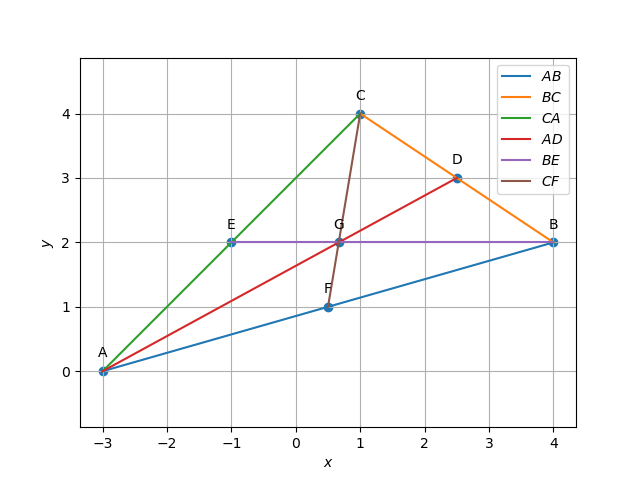
\includegraphics[width=\columnwidth]{/sdcard/geometry/geometry/figs/med2.png}
\caption{$G$ is the centroid of triangle $ABC$}
\label{fig:Triangle101}
\end{figure}



%Question 1.2.4:
\item Verify that 
		\begin{align}
			\frac{BG}{GE} = 
			\frac{CG}{GF} =
			\frac{AG}{GD} =2 
		\end{align}\\
Question 1.2.4:Verify that 
\begin{align}
		\frac{BG}{GE} = 
		\frac{CG}{GF} =
		\frac{AG}{GD} = 2 
\end{align}
\solution In order to verify the above equation we first need to find $\vec{G}$.$\vec{G}$ is the intersection of $BE$ and $CF$,Using the value of $\vec{G}$ from (1.2.3).
\begin{align}
		\vec{G} = \myvec{\frac{2}{3}\\2}
\end{align}
Also,We know that $\vec{D}, \vec{E}$ and $\vec{F}$ are midpoints of $BC, CA$ and $AB$ respectively from (1.2.1).
\begin{align}
		\vec{D} = \myvec{\frac{5}{2} \\ 3},\,
		\vec{E} = \myvec{-1 \\ 2},\,
		\vec{F} = \myvec{\frac{1}{2}\\ 1}
\end{align}
\begin{enumerate}
\item Calculating the ratio of $BG$ and $GE$,
\begin{align}
		\label{eq:tri-pts/4} \vec{G}-\vec{B} &= \myvec{\frac{-10}{3} \\ 0} \\
		\label{eq:tri-pts/5} \vec{E}-\vec{G} &= \myvec{\frac{-5}{3} \\ 0} \\
		\label{eq:tri-pts/6} \norm{\vec{G}-\vec{B}} &= \sqrt{\brak{\frac{-10}{0}}^2 + \brak{\frac{-5}{0}}^{2}}  \\
		\label{eq:tri-pts/7} \norm{\vec{E}-\vec{G}} &= \sqrt{\brak{\frac{-13}{6}}^2 + \brak{\frac{-4}{3}}^2} &= \frac{\sqrt{233}}{6} \\
		\label{eq:tri-pts/8}\frac{BG}{GE} &= \frac{\norm{\vec{G}-\vec{B}}}{\norm{\vec{E}-\vec{G}}}&= 2  
\end{align}		
\end{enumerate}

From \eqref{eq:tri-pts/8}, \eqref{eq:tri-pts/13}, \eqref{eq:tri-pts/18}
\begin{align}
		\frac{BG}{GE} = 
		\frac{CG}{GF} =
		\frac{AG}{GD} = 2
\end{align}
Hence verified.



%Question 1.2.5:
\item Show that $\vec{A}, \vec{G}$ and $\vec{D}$ are collinear.\\
\solution 
Given that,
\begin{align}
    \vec{A} = \myvec{-3\\0}
    \quad
    \vec{B} &= \myvec{4\\2}
    \quad
    \vec{C} = \myvec{1\\4}
\end{align}
We need to show that points $\vec{A},\vec{D},\vec{G}$ are collinear.
From Problem 1.2.3 We know that, The point $\vec{G}$ is 
\begin{align}
    \vec{G} &=\myvec{\frac{2}{3}\\ 2}
\end{align}
And from Problem 1.2.1 We know that, The point $\vec{D}$ is 
\begin{align}
    \vec{D} &=\myvec{\frac{5}{2}\\ 3}
\end{align}
In Problem 1.1.3, There is a theorem/law mentioned i.e.,

Points $\vec{A},\vec{D},\vec{G}$ are defined to be collinear if 
\begin{align}
    \text{rank}\myvec{
    1 & 1 & 1\\
    \vec{A} & \vec{D} & \vec{G} \\
    } &= 2 
\end{align} 
Using the above law/Theorem Let
\begin{align}
    \vec{R}&=\myvec{
    1 & 1 & 1
    \\
    -3 & \frac{5}{2} & \frac{2}{3}
    \\
    0 & 3 & 2
    } 
\end{align} 
The matrix $\vec{R}$ can be row reduced as follows,
\begin{align}
    \label{eq:mat_row_operations}
    \myvec{
    1 & 1 & 1
    \\
    -3 & \frac{5}{2} & \frac{2}{3}
    \\
    0 & 3 & 2
    }
     \xleftrightarrow[]{}
    \myvec{
    1 & 1 & 1
    \\
    0 & 1 & \frac{2}{3}
    \\
    0 & 0 & 0
    }
\end{align}
Rank of above matrix is 2.\\
Hence, we proved that that points $\vec{A},\vec{D},\vec{G}$ are collinear.



%Question 1.2.6:
\item Verify that 
		\begin{align}
			\vec{G}=\frac{\vec{A}+\vec{B}+\vec{C}}{3}
		\end{align}
$\vec{G}$ is known as the {\em centroid} of $\triangle ABC$.\\
Verify that\\
\begin{align}
 \vec{G}=\frac{\vec{A}+\vec{B}+\vec{C}}{3}   
\end{align}
$\vec{G}$ is known as the \underline{centroid} of $\triangle$ABC 
SOLUTION:\\
let us first evaluate the R.H.S of the equation
\begin{equation}
\begin{split}
\label{eq:centroid}
    \vec{G}&= \frac{\myvec{-3\\0}+\myvec{4\\2}+\myvec{1\\4}}{3}\\   
     &= \myvec{\frac{2}{3}\\ 2}
\end{split}
\end{equation}
Hence verified.


%Question 1.2.7: 
\item Verify that 
		\begin{align}
\vec{A}-\vec{F}=\vec{E}-\vec{D}
		\end{align}
The quadrilateral $AFDE$ is defined to be a parallelogram.\\
Question : Verify that 
\begin{align}
	\vec{A}-\vec{F} = \vec{E}-\vec{D}
\end{align}
The quadrilateral $AFDE$ is defined to be parallelogram
\\ \solution 
Given that,
\begin{align}
    \vec{A} = \myvec{-3\\0}
    \quad
    \vec{B} &= \myvec{4\\2}
    \quad
    \vec{C} = \myvec{1\\4}
\end{align}
From Problem 1.2.1 We know that, The point $\vec{D},\vec{E},\vec{F}$ is 
\begin{align}
    \vec{D} = \myvec{\frac{5}{2}\\ 3 }
    \quad
    \vec{E} &= \myvec{-1\\2}
    \quad
    \vec{F} = \myvec{\frac{1}{2}\\ 1}
\end{align}
Evaluating the R.H.S of the equation
\begin{align}
    \vec{A}-\vec{F}&=\myvec{ \frac{-7}{2} \\ -1 }
\end{align} 
Evaluating the L.H.S of the equation
\begin{align}
    \vec{E}-\vec{D}&=\myvec{\frac{-7}{2} \\ -1 }
\end{align}
Hence verified that, R.H.S = L.H.S i.e.,
\begin{align}
	\vec{A}-\vec{F} = \vec{E}-\vec{D}
\end{align}
From the fig\ref{fig:Triangle}, It is verified that $AFDE$ is a parallelogram
\begin{figure}
\centering
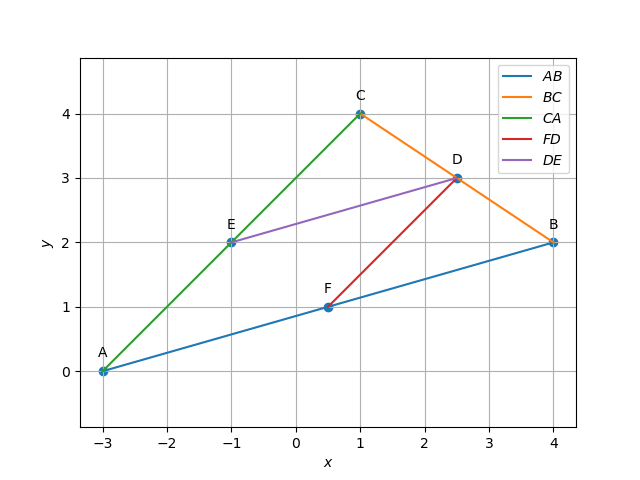
\includegraphics[width=\columnwidth]{/sdcard/geometry/geometry/figs/prm.png}
\caption{$AFDE$ form a parallelogram in triangle ABC}
\label{fig:Triangle}
\end{figure}
\end{enumerate}














%\input{subsec/median}
%\section{Altitude}
%\section{Perpendicular Bisector}
%\section{Angle Bisector}

\end{document}
{

%\section{Altitude}
%\section{Perpendicular Bisector}
%\section{Angle Bisector}

\end{document}
{

%\section{Altitude}
%\section{Perpendicular Bisector}
%\section{Angle Bisector}

\end{document}
{

%\section{Altitude}
%\section{Perpendicular Bisector}
%\section{Angle Bisector}
\end{document} 
